\begin{frame}{Inertia}
  \begin{mycolumns}

    \begin{column}{.5\textwidth}\includegraphics[width=4in]{ch01/figs/convertible}\end{column}

    \begin{column}{.5\textwidth}
      \dq

      Right or wrong? Motion isn't relative.
      When you're driving in a convertible with the top down, the wind in
      your face is an observable physical effect of your motion.
    \end{column}
  \end{mycolumns}

  \cred{Cadillac: redrawn from a photo by That Hartford Guy, CC-BY-SA}

\end{frame}


\begin{frame}{Inertia}
  \begin{mycolumns}

    \begin{column}{.4\textwidth}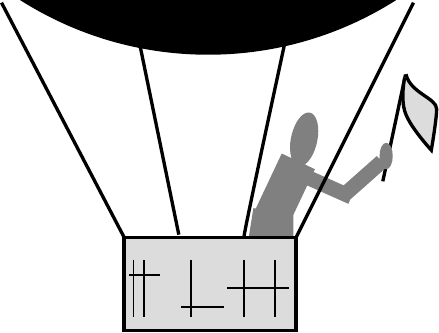
\includegraphics[width=4in]{ch01/figs/flag-in-balloon}\end{column}

    \begin{column}{.6\textwidth}
      \dq

You are a passenger in the open basket hanging under a
helium balloon. The balloon is being carried along by the
wind at a constant velocity. If you are holding a flag in
your hand, will the flag wave? If so, which way?

\cred{Based on a question from PSSC Physics}


    \end{column}
  \end{mycolumns}
\end{frame}

\begin{frame}{Inertia}
  \begin{mycolumns}

    \begin{column}{.7\textwidth}
\includegraphics[width=7in]{ch01/figs/rocket-sled}\end{column}

    \begin{column}{.3\textwidth}
      \dq

      This Air Force doctor volunteered to ride a rocket sled as
      a medical experiment. Doesn't this show that motion has a physical effect on him?

      \cred{Photo of rocket sled: U.S.~Air Force, public domain work of the U.S.~Government.}
    \end{column}
  \end{mycolumns}
\end{frame}

\begin{frame}{Inertia}
  \begin{mycolumns}

    \begin{column}{.4\textwidth}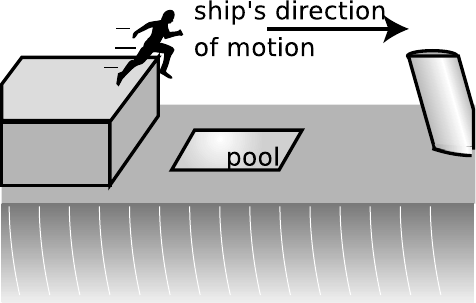
\includegraphics[width=4in]{ch01/figs/cruise-ship}\end{column}

    \begin{column}{.6\textwidth}
      \dq

      A passenger on a cruise ship finds, while the ship is docked, that
      he can leap off of the upper deck and just barely make it into the pool
      on the lower deck. If the ship leaves dock and is cruising rapidly, will this
      adrenaline junkie still be able to make it?
    \end{column}
  \end{mycolumns}
\end{frame}
